\section{Концепция агентно-ориентированного программирования}
\subsection{Историческое развитие агентно-ориентированного подхода}
История теории агентов неразрывно связана с общим контекстом становления кибернетики, теории автоматов, искусственного интеллекта как научных дисциплин, моделирующих поведение искусственных и биологических сущностей в условиях некоторой внешней среды.

Фундаментальным базисом для формирования агентно-ориентированных представлений послужили труды А. Н.~Колмогорова по теории информации и алгоритмической сложности объектов, И.~Пригожина, И.~Стенгерс, Г.~Хакена по теории самоорганизации и эволюции открытых систем, У.Р.~Эшби по моделям гомеостазиса и разнообразию систем, А.~Беркса по клеточным автоматам и моделированию эволюционных систем, Дж.~Холланда и Д.~Гольдберга по генетическим алгоритмам.

Большую роль в становлении агентно-ориентированного подхода сыграли работы Карла Хьюитта в области открытых систем и теории акторов. Предложив в 1969 г. язык PLANNER для доказательства теорем, К.~Хьюитт раскрыл значение процессов коммуникации и управления в организации и понимании рассуждений. Отойдя от рассмотрения управления как последовательности актов выбора, он ввел вариант распределенной системы, в которой структуры управления трактовались как <<образцы прохождения сообщений>>, циркулирующих между активными объектами, названными им акторами. По К.~Хьюитту, актор~--- это программный агент, имеющий свой почтовый адрес и обладающий определенным поведением. В результате появилось семейство языков для программирования задач параллельного искусственного интеллекта, которые стали первыми средствами реализации мультиагентных систем, осуществляющих коммуникацию путем посылки асинхронных сообщений.

Первые западные практические разработки агентно-ориентированных систем  относятся к 70-м годам прошлого века и связаны с именами В.~Лессера и Д.~Лената. Их работы привели к созданию архитектуры «классной доски» (blackboard) и легли в основу многих дальнейших разработок по организации коммуникации между агентами. Исследуя проблематику автоматического понимания речи, они воспользовались метафорой <<классной доски>>, полагая, что решение проблемы обычно требует заранее не запланированных обращений к источникам знаний. При этом структура управления процессом коммуникации предварительно не определена. Деятельность источников знаний связана с доставкой, модификацией и извлечением объектов с <<классной доски>>, т.е. из зоны совместной работы в базе данных, где модель предметной области структурирована как пространство гипотез и решений. Специальное управляющее устройство разрешает конфликты доступа к <<классной доске>>, возникающие между агентами и неявно организует их совместную работу.

Другой тип управления взаимодействием агентов был предложен Д.~Ленатом и К.~Хьюиттом в системе PUPS, где была реализована идея решения задачи группой агентов (специалистов), именуемых <<beings>> (<<сущности>>). Эти <<сущности>> стремятся синтезировать особого специалиста по формированию концепций, способного самостоятельно решить задачу. Сами специалисты постоянно меняются в процессе решения задачи и не могут быть отнесенык классическим источникам знаний. Каждый специалист моделируется подобно фрейму множеством пар <<атрибут -- значение>> и может обращаться за сведениями к другим специалистам, не зная их лично.

В начале 80-х годов Р.~Смит разработал модель распределенного решения задач под названием «протокол контрактной сети», которая получила большую известность и стандартизована FIPA. Модель использует метафору переговоров между автономными интеллектуальными агентами и основана на протоколе рыночных торгов. Имеются три типа агентов: агент-менеджер, агент-исполнитель, агент-подрядчик. Агент-менеджер распространяет объявление о задании и определяет исходную цену, а агенты—потенциальные исполнители предлагают свои услуги, посылая свои варианты цен, и участвуют в конкурсе на определение наилучших предложений по исходному заданию. Затем агент-менеджер отбирает наилучшие предложения и заключает соглашение с выбранными агентами-исполнителями, которые становятся агентами-подрядчиками.

Одной из важнейших работ начала 90-х г.г. стала статья И.~Шоэма <<Агентно-ориентированное программирование>> (АОП). В ней описан социальный взгляд на организацию вычислений, связанный с взаимодействием агентов в процессе вычислений. При этом агент рассматривается как <<прозрачный ящик>> и моделируются такие его <<внутренние переменные>> как мотивы, убеждения, обязательства, способности к выработке и принятию решений. Мотивы агента лежат в основе его решений, а убеждения определяют логические ограничения на них. Общение агентов осуществляется с помощью протоколов коммуникации.
Система АОП должна включать следующие базовые компоненты: ограниченный формальный язык с соответствующими синтаксисом и семантикой для описания внутреннего состояния агента; язык программирования для спецификации агентов; агентификатор, преобразующий нейтральные компоненты в программируемых агентов.

При уточнении отличий АОП от классических направлений искусственного интеллекта удобно опираться на представления развитые школой объектно-ориентированного программирования (ООП). Объект имеет имя, собственные данные и процедуры. Он может состоять из нескольких определенных объектов и в свою очередь быть частью более крупного объекта. Все действия в ООП выполняются через сообщения. В целом, понятие объекта определяется с помощью трех ключевых признаков: инкапсуляция, наследование, полиморфизм.

При разработке программного обеспечения на основе ООП используется модель реального мира вида <<объект-класс-сообщение>>. Объекты не могут анализировать свое поведение, определять характер связей с другими объектами и самостоятельно формировать цели.

Так же и акторы не могут проводить рассуждения о содержании этих сообщений. Модель акторов организована, исходя из двух простых принципов: посылки сообщений и локальной обработки. На локальном уровне актор содержит три составляющих: знания о своей среде; знания о других акторах; множество данных и действий. Эти составляющие определяют его локальное поведение в зависимости от поступающего сообщения. Когда актор получает некоторое сообщение, он может передавать его другим акторам. Помимо этого, актор способен создавать новых акторов и изменять свое внутреннее состояние.

Однако, в отличие от объекта, агент может принять на себя определенные обязательства или, наоборот, отказаться от выполнения некоторой работы, мотивируя это отсутствием компетентности, занятостью другой задачей и т.п. В то же время, агент может выполнять такие действия как порождение, подавление и замена других агентов, активизация функций (как своих, так и у других агентов), активизация сценария деятельности, запоминание текущего состояния других агентов и пр. Все это наглядно показывает, что агент, будучи <<активным объектом>> или <<искусственным деятелем>>, формирующим свое собственное поведение, находится на более высоком уровне сложности по отношению к традиционным объектам в ООП.

\subsection{Агентно-ориентированный подход к программированию}
Агентно-ориентированный подход (в дальнейшем АОП) к программированию~---  разновидность представления программ или парадигма программирования, в которой основополагающими концепциями являются понятия агента и его ментальное поведение, зависящее от среды, в которой он находится. Концепция была предложена Шохемом в 1990 г. Определение парадигмы, данное автором:
"Эту новую парадигму программирования вполне разумно назвать рациональным программированием. Точно так же, как объектно-ориентированное программирование сдвинуло парадигму с написания процедур к созданию объектов, рациональное программирование сдвинуло парадигму с создания информационных объектов к созданию мотивированных агентов."

Агентный подход является следующим этапов в разработке приложений с архитектурой взаимодействующих компонентов после классической клиент-серверного подхода, позволяя сохранить его положительные черты и преодолеть большинство его недостатков. При использовании агентного подхода приложение логически делится на множество компонентов, имеющих значительную автономности и способных взаимодействовать между собой.

Использование агентов при сборе, поиске и анализе информации имеет ряд преимушеств, основные из которых сводятся к следующему:
\begin{itemize}
\item агенты могут обеспечить пользователю доступ к любым Интернет-сервисам и сетевым протоколам;
\item агент может получать и решать новые задачи, будучи уже занятым решением других задач, за счет возможности копировать себя и передавать своим копиям новые задачи;
\item агенты могут осуществлять поиск по заданию пользователя автономно, после отключения его от сети, и уведомляя о полученных результатах при следующем его подключении;
\item мобильность позволяет агентам проводить поиск (обработку) информации непосредственно по месту её размещения, что увеличивает скорость и точность обработки, а также уменьшает загрузку сети;
\item агенты могут создавать собственную базу информационных ресурсов, которая может постоянно обновляться и расширяться с каждым проделанным заданием;
\item возможность агентов сотрудничать друг с другом позволяет использовать их опыт в процессе выполнения задачи;
\item агенты могут осуществлять мониторинг источников информации, уведомляя пользователя о появлении новых данных;
\item агенты могут адаптироваться под предпочтения и желания пользователя;
\item агенты могут работать с информацией, учитывая её контекст;
\item агенты могут работать с информацией интеллектуально, например, используя словари, тезаурусы, онтологии и др., а также средства вывода релевантной информации, не представленной явно ни в запросе, ни в найденных документах.
\end{itemize}

Кроме того, использование агентных технологий:
\begin{itemize}
\item упростит процессы размещения (deployment) программного обеспечения в условиях сети, автоматизируя процессы перемещения программного кода, его установки и конфигурирования;
\item упростит процессы обновления программного кода, заменяя неактивные в данный момент компоненты новыми версиями, сохраняя при этом ассоциированные с компонентом данные, совершенно прозрачно для работы всей системы в целом;
\item упростит удаленный доступ и управление в условиях сети, в том числе с использованием мобильных устройств, таких как планшетные компьютеры и сотовые телефоны;
\item значительно уменьшит сетевой трафик и общую избыточность информации за счет возможности непосредственного перемещения кода агента к обрабатываемым данным, вместо перемещения самих данных, как в случае использования клиент-серверного подхода.
\item даст возможность балансировать нагрузку между несколькими вычислительными ресурсами и вести параллельную обработку данных за счет возможности асинхронной коммуникации между агентами и возможности перемещения кода агента по сети;
\item значительно сократит время и затраты на администрирование;
\item упростит разработку программного обеспечения за счет широких возможностей повторного использования уже существующего программного обеспечения и параллельной разработки ПО.
\end{itemize}

\subsection{Понятие агента и его свойства}
Э.~Таненбаум~--- всемирно известный специалист в области информационных технологий~--- определяет программный агент как автономный процесс, способный реагировать на среду исполнения и вызывать изменения в среде исполнения, возможно, в кооперации с пользователями или другими агентами. Таненбаум также приводит классификацию агентов, в которой выделяются следующие основные типы.
\begin{figure}[h]
\center{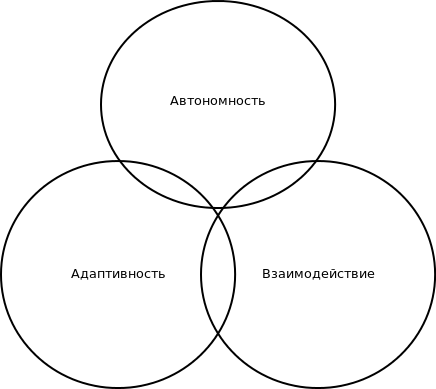
\includegraphics[width=0.6\linewidth]{tanenbaum-agent}}
\caption{Образующие свойства агента по Э.~Таненбауму}
\label{1:tanenbaum-agent}
\end{figure}

Стационарные и мобильные агенты. Мобильные агенты способны перемещаться с одного узла ВС на другой. Стационарные~--- прикреплены к конкретному вычислительному узлу.
Кооперативные и конкурирующие. Кооперативный агент~--- способный объединяться с другими агентами для решения общей задачи. Конкурирующий~--- способен конкурировать с другими агентами с целью защиты интересов своего владельца (например, торговые агенты на бирже).

Агенты могут применяться при решении следующих задач:
\begin{itemize}
\item мобильные вычисления (миграция агентов может поддерживаться не только между постоянно подсоединенными к сети узлами, но и между мобильными платформами, подключаемыми к постоянной сети на некоторые промежутки времени и возможно по низкоскоростным каналам). Клиент подсоединяется к постоянной сети на короткий промежуток времени с мобильной платформы, отправляет агента для выполнения задачи и отсоединяется; затем клиент подсоединяется к другой точке сети и забирает результаты работы агента. Второй вариант~--- сервер, на который должен переместиться агент, подсоединяется к сети, а затем отсоединяется. В этом случае агент должен уметь переместиться на такой временно подсоединяемый сервер и вернуться в постоянную сеть;
\item задачи управления информацией:
\begin{itemize}
\item поиск информации (один человек не в состоянии найти необходимую ему информацию и проанализировать ее~--- использование агента, который странствует по сети в поисках информации, лучше всего удовлетворяющей потребности человека); поисковые агенты содержат сведения о различных информационных источниках (включая тип информации, способ доступа к ней, а также такие характеристики информационного источника, как надежность и точность данных);
\item отбор (обработка) информации. Из всех данных, приходящих к клиенту, выбирают только те данные, которые могут быть интересны клиенту. Используются в комбинации с поисковыми агентами (сначала поиск, затем~--- отбор);
\item мониторинг данных. Извещение пользователя об изменениях в различных источниках данных в реальном времени (например, мобильный агент перемещается на вычислительный узел, на котором расположен источник данных; это эффективнее, чем использовать статического агента, посылающего запросы источнику данных);
\item универсальный доступ к данным. Агенты–посредники для работы с различными источниками данных, имеющие механизмы для взаимодействия друг с другом (например, агент создает несколько агентов, каждый из которых работает со своим источником данных).
\end{itemize}
\end{itemize}

С.~Франклин и А.~Грэссер в 1996 году предложили следующее обобщенное определение агента: Автономный агент~--- это система, находящаяся внутри окружения и являющаяся его частью, воспринимающая это окружение (его сигналы) и воздействующая на окружение для выполнения собственной программы действий.
\begin{figure}[h]
\center{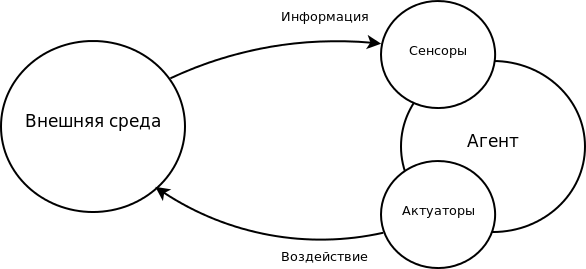
\includegraphics[width=0.8\linewidth]{franklin-agent}}
\caption{Модель автономного агента С.~Франклина и А.~Грэссера}
\label{1:franklin-agent}
\end{figure}

Можно выделить следующие основные составляющие автономного агента:
\begin{enumerate}
\item Сенсоры: блоки агента, обеспечивающие получение информации об окружающей среде и других агентах;
\item Актуаторы: блоки агента, обеспечивающие воздействие на окружающую среду.
\end{enumerate}

Автономный агент должен обладать следующими свойствами:
\begin{itemize}
\item реактивность;
\item автономность;
\item целенаправленность;
\item коммуникативность.
\end{itemize}

Свойство реактивности означает, что агент временами отвечает на изменения в окружении. Агент имеет сенсоры, с помощью которых получает информацию от окружения. Сенсоры могут быть самыми различными. Это могут быть микрофоны, воспринимающие акустические сигналы и преобразующие их в электрические, видеокарты захвата изображений, клавиатура компьютера или общая область памяти, в которую окружение помещает данные и из которой программный агент берет данные для вычислений. Не все изменения окружения становятся известными (доступными) сенсорам агента. Это вполне естественно. Ведь и человек не воспринимает звуки частотой свыше 30 кГц, радиоволны и т.д. Таким образом, окружение не является полностью наблюдаемым для агента. Аналогично, агент воздействует на окружение путем разнообразных исполнительных механизмов, включая общую память. Разумеется, степень воздействия как и степень восприятия является ограниченной. Агент может перевести окружение из некоторого состояния в некоторое другое, но не из любого в любое.

Свойство автономности означает, что агент является самоуправляющимся, сам контролирует свои действия. Программный агент, находящийся на некотором сервере, обладает возможностью <<самозапуска>>. Он не требует от пользователя каких-либо специальных действий по обеспечению его старта.

Свойство целенаправленности означает, что у агента имеется определенная цель и его поведение (воздействие на окружение) подчинено этой цели, а не является простым откликом на сигналы из окружения. Иначе говоря, агент является управляющей системой, а не управляемым объектом.

Свойство коммуникативности означает, что агент общается с другими агентами (включая людей), используя для этого некоторый язык. Это не обязательно единый язык для всех агентов. Достаточно, чтобы у пары общающихся агентов был общий язык. Язык может быть сложным как, например, естественный язык. Но может быть и примитивным: обмен числами или короткими словами.

В отдельную категорию интеллектуальных агентов выделяют автономные агенты, обладающей свойством обучаемости. Свойство обучаемости означает, что агент может корректировать свое поведение, основываясь на предыдущем опыте. Это не просто накопление в памяти параметров окружения, т.е. использование исторических данных, но сопоставление истории собственных действий с историей их влияние на окружение, и изменение в связи с этим своей программы действий.

\subsection{Агентные (мультиагентные) системы}
Мультиагентной системой (МАС) называется система, решающая одну задачу несколькими агентами методом передачи знаний и задач (действий) между агентами. Ее агенты ограничены (не знают о всей системе) и децентрализованы (не управляют всей системой).

Многоагентные системы могут быть использованы для решения таких проблем, которые сложно или невозможно решить с помощью одного агента или монолитной системы.

В таких системах необязательно все агенты взаимодействуют (общаются) между собой. В крайнем случае, общения нет вообще. Такие системы назовем дискретными мультиагентными системами. Второй крайний случай~--- каждый агент общается с каждым. Такую систему назовем полносвязной муль тиагентной системой.

Мультиагентная система, действующая как единый агент, должна характеризоваться и некоторой общей для всех субагентов целью и координацией действий по достижению этой цели.

Поскольку встречаются и другие ситуации, когда агенты не связаны столь тесно, то такие системы можно назвать обществами агентов. Отсутствие единой цели, однако, не отрицает возможного группового поведения агентов. Но оно является, скорее, эпизодическим, чем систематическим.

Важным отличием мультиагентной системы от программы или одного агента является то, что входящие в систему программные агенты (по крайней мере, некоторые) не были спроектированы специально для этой системы. Может быть, это~--- повторно используемые агенты, или агенты, разработанные для решения более универсальных задач. В этих случаях агенты имеют собственные цели, не совпадающие полностью с целями системы (организации), но совместимые с ними. Тем не менее, они могут быть полезны друг другу для решения стоящих перед ними задач и, поэтому, очень важным для них с этой точки зрения является свойство коммуникативности.

С организационной точки зрения существуют общие цели всего сообщества, и эти общие цели выражаются, прежде всего, в ролях (которые играют агенты) и нормах взаимодействия.

Исследования в области систем поддержки принятия решений (DSS) в последние годы все больше переходят от создания систем в виде традиционного <<ящика с инструментами>> (toolbox) к парадигме сотрудничества и интеграции независимых приложений. Быстро растущая область исследований и нтеллектуальных агентов и мультиагентных систем предлагает возможности создания более эффективных систем на основе единого подхода.

Программирование МАС можно разделить на:
\begin{itemize}
\item примитивы агента;
\item организацию (архитектура и функции);
\item цели (состояние агента во времени, влияние выполнения задачи на состояние, как достигаются цели и что приосходит если их нельзя достигнуть);
\item окружение агентов;
\item межагентное взаимодействие;
\end{itemize}

\subsection{Стандарты агентных систем}
\begin{figure}[h]
\center{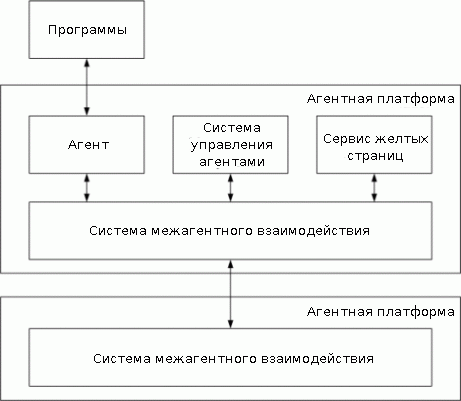
\includegraphics[width=0.6\linewidth]{fipa}}
\caption{Архитектура FIPA}
\label{1:fipa}
\end{figure}

В настоящее время ведется активная работа над разработкой стандартов, описывающих функционирование агентов и агентных систем~--- одним из ведущих является стандарт Фонда интеллектуальных программных агентов~--- FIPA.

FIPA предлагает коллекцию стандартов, направленных на продвижение гетерогенных агентов и сервисов, которые они предоставляют. Эти спецификации в общих чертах описывают коммуникационные языки агентов, услуги агентов и онтологии поддержки агентов в мультиагентных системах.

FIPA~--- является международным стандартом, который описывает функции агентных технологий, и совместимость стандартов агентов с другими технологиями. FIPA стандарты были организованы специально для агентов и многоагентных систем, и были официально приняты 8 июня 2005 года. FIPA сыграл решающую роль в развитии стандартов для агентов и их взаимодействия друг с другом, услуг, которые они могут представлять.

Стандарты FIPA включает в себя описания основных компонентов, которые должны составлять агентные системы, а также окружающую агентов среду и способы связи между собой. Также, для того чтобы облегчить связь между агентными системами разных разработчиков, FIPA стандарты описывают стандартизированные интерфейсы, которыми должны пользоваться агенты для связи друг с другом~--- Agent Communication Language. По FIPA агенты могут обмениваться сообщениями в трех протоколах~--- WAP, IIOP и  HTTP. Также в стандартах FIPA описывается диспетчер задач и диспетчер сообщений~--- два обязательных для агентной платформы сервиса, которые также реализованы в JADE. Первый из них необходим для выбора поведений, которые агент выполняет параллельно. Второй нужен для содержания очереди сообщений.
